\newpage
\section{Results for Delay of 0}

\begin{figure}[hb]
    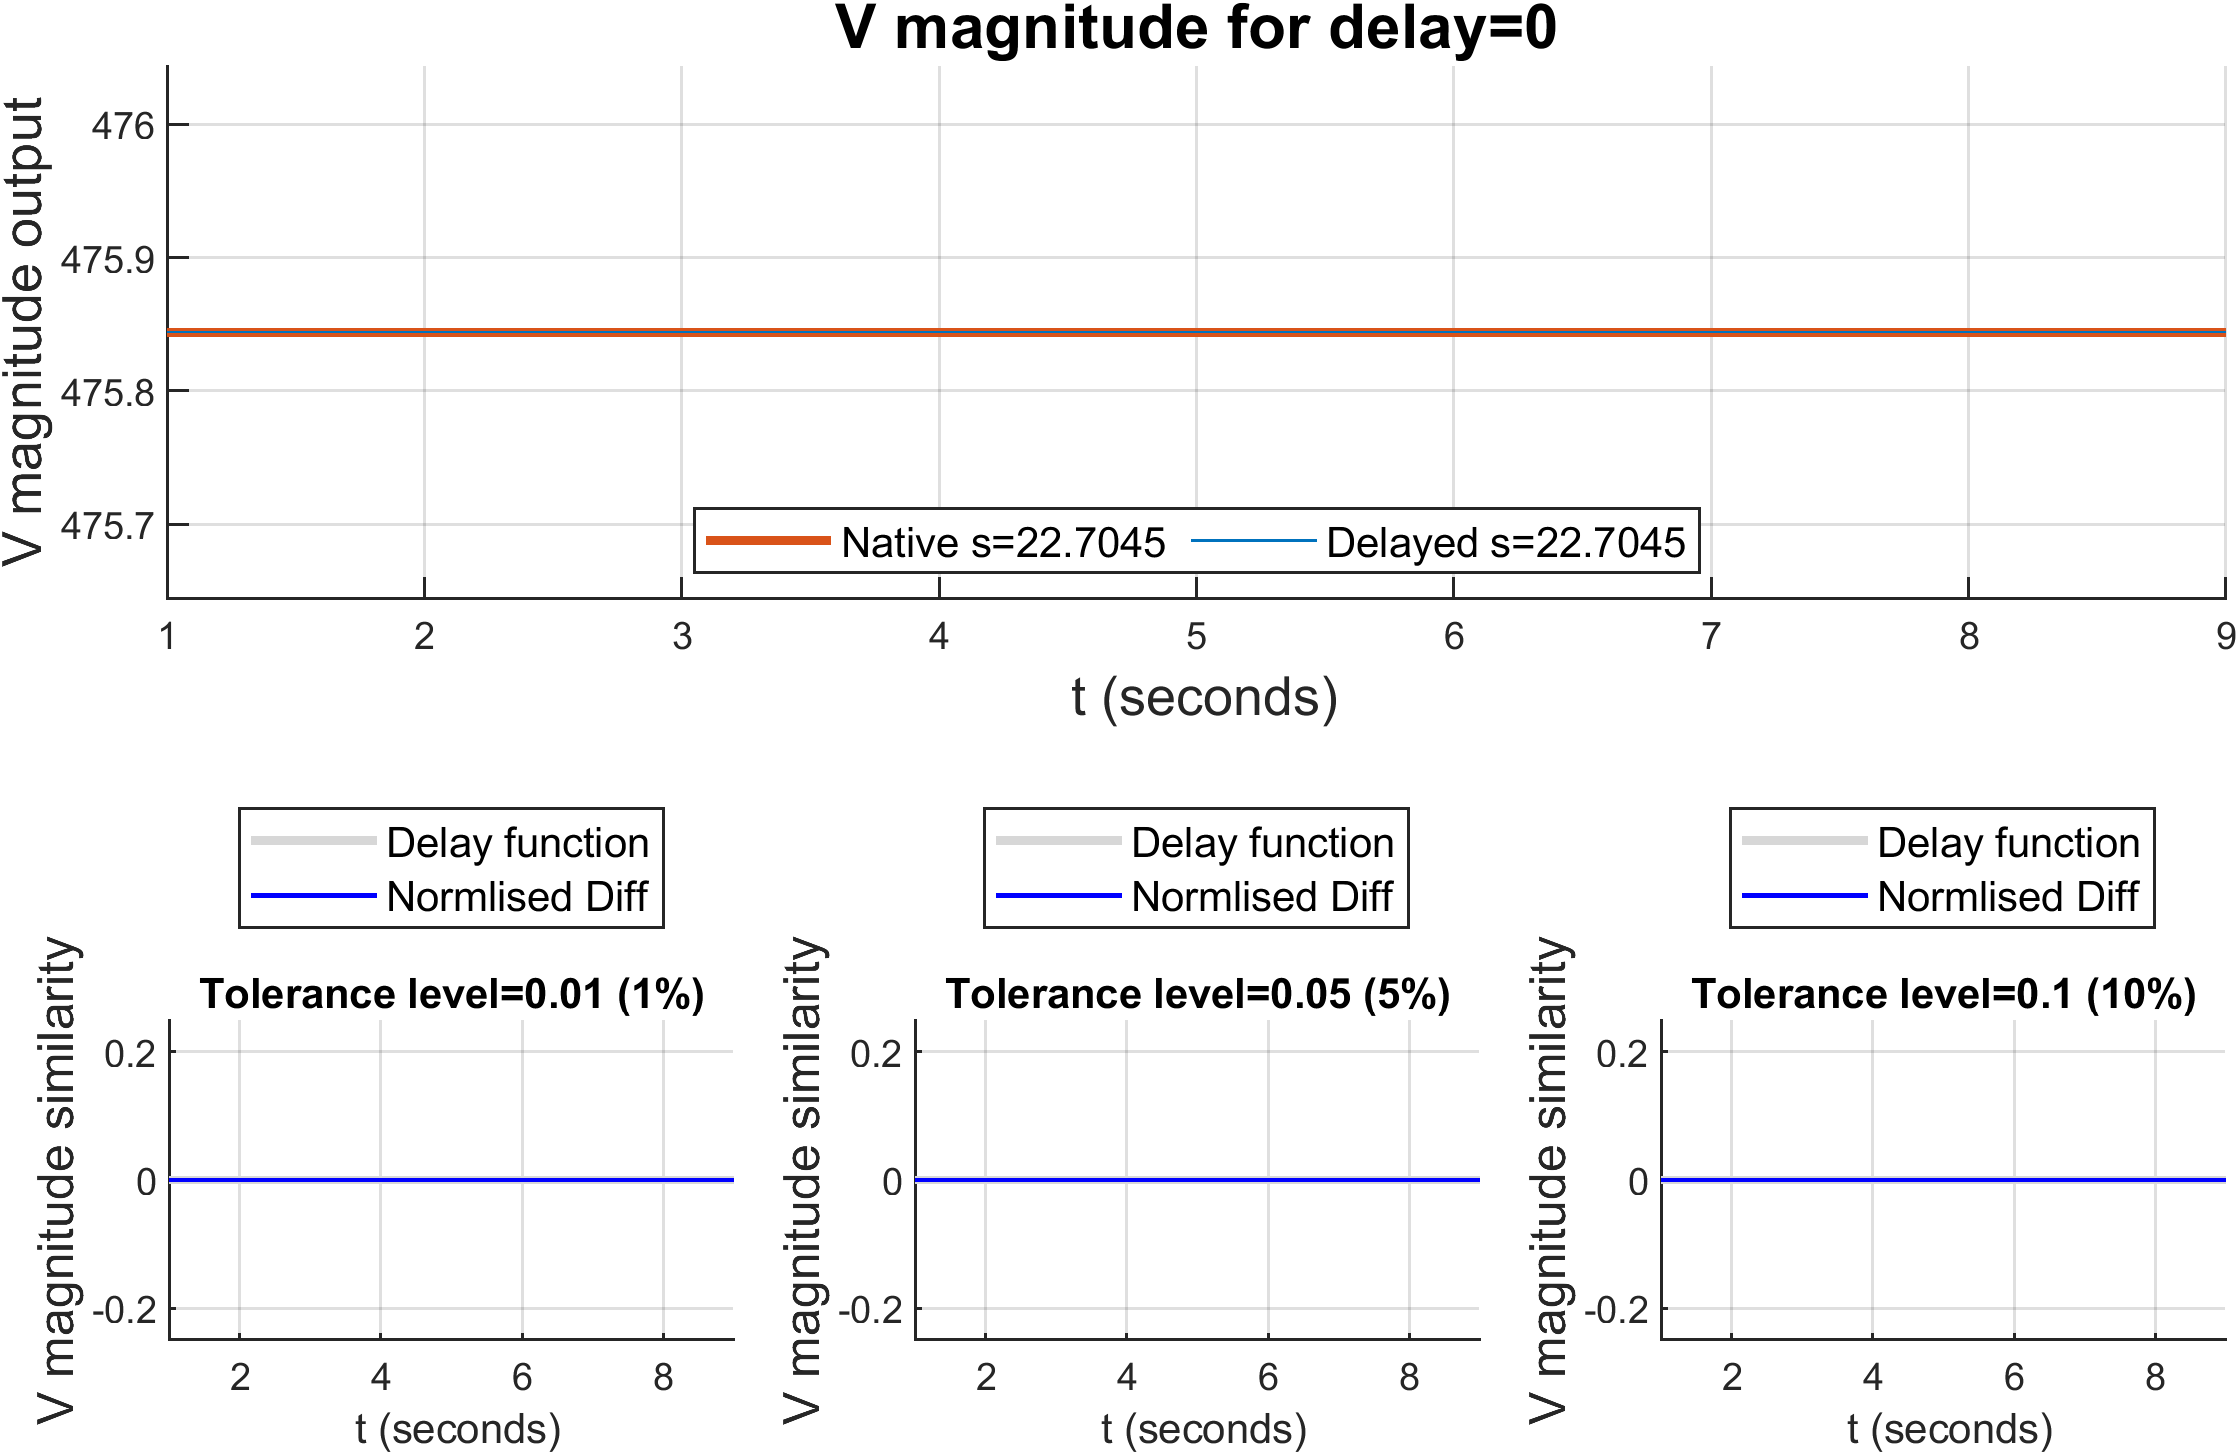
\includegraphics[width=0.95\textwidth]{\locateResults/DelayOf_0/Zero_vMagnitude.png}    
    \caption{Ascending delay combined output}
    \label{fig:PMUsim_Zero_iMagn}
\end{figure}

\begin{figure}[hb]
    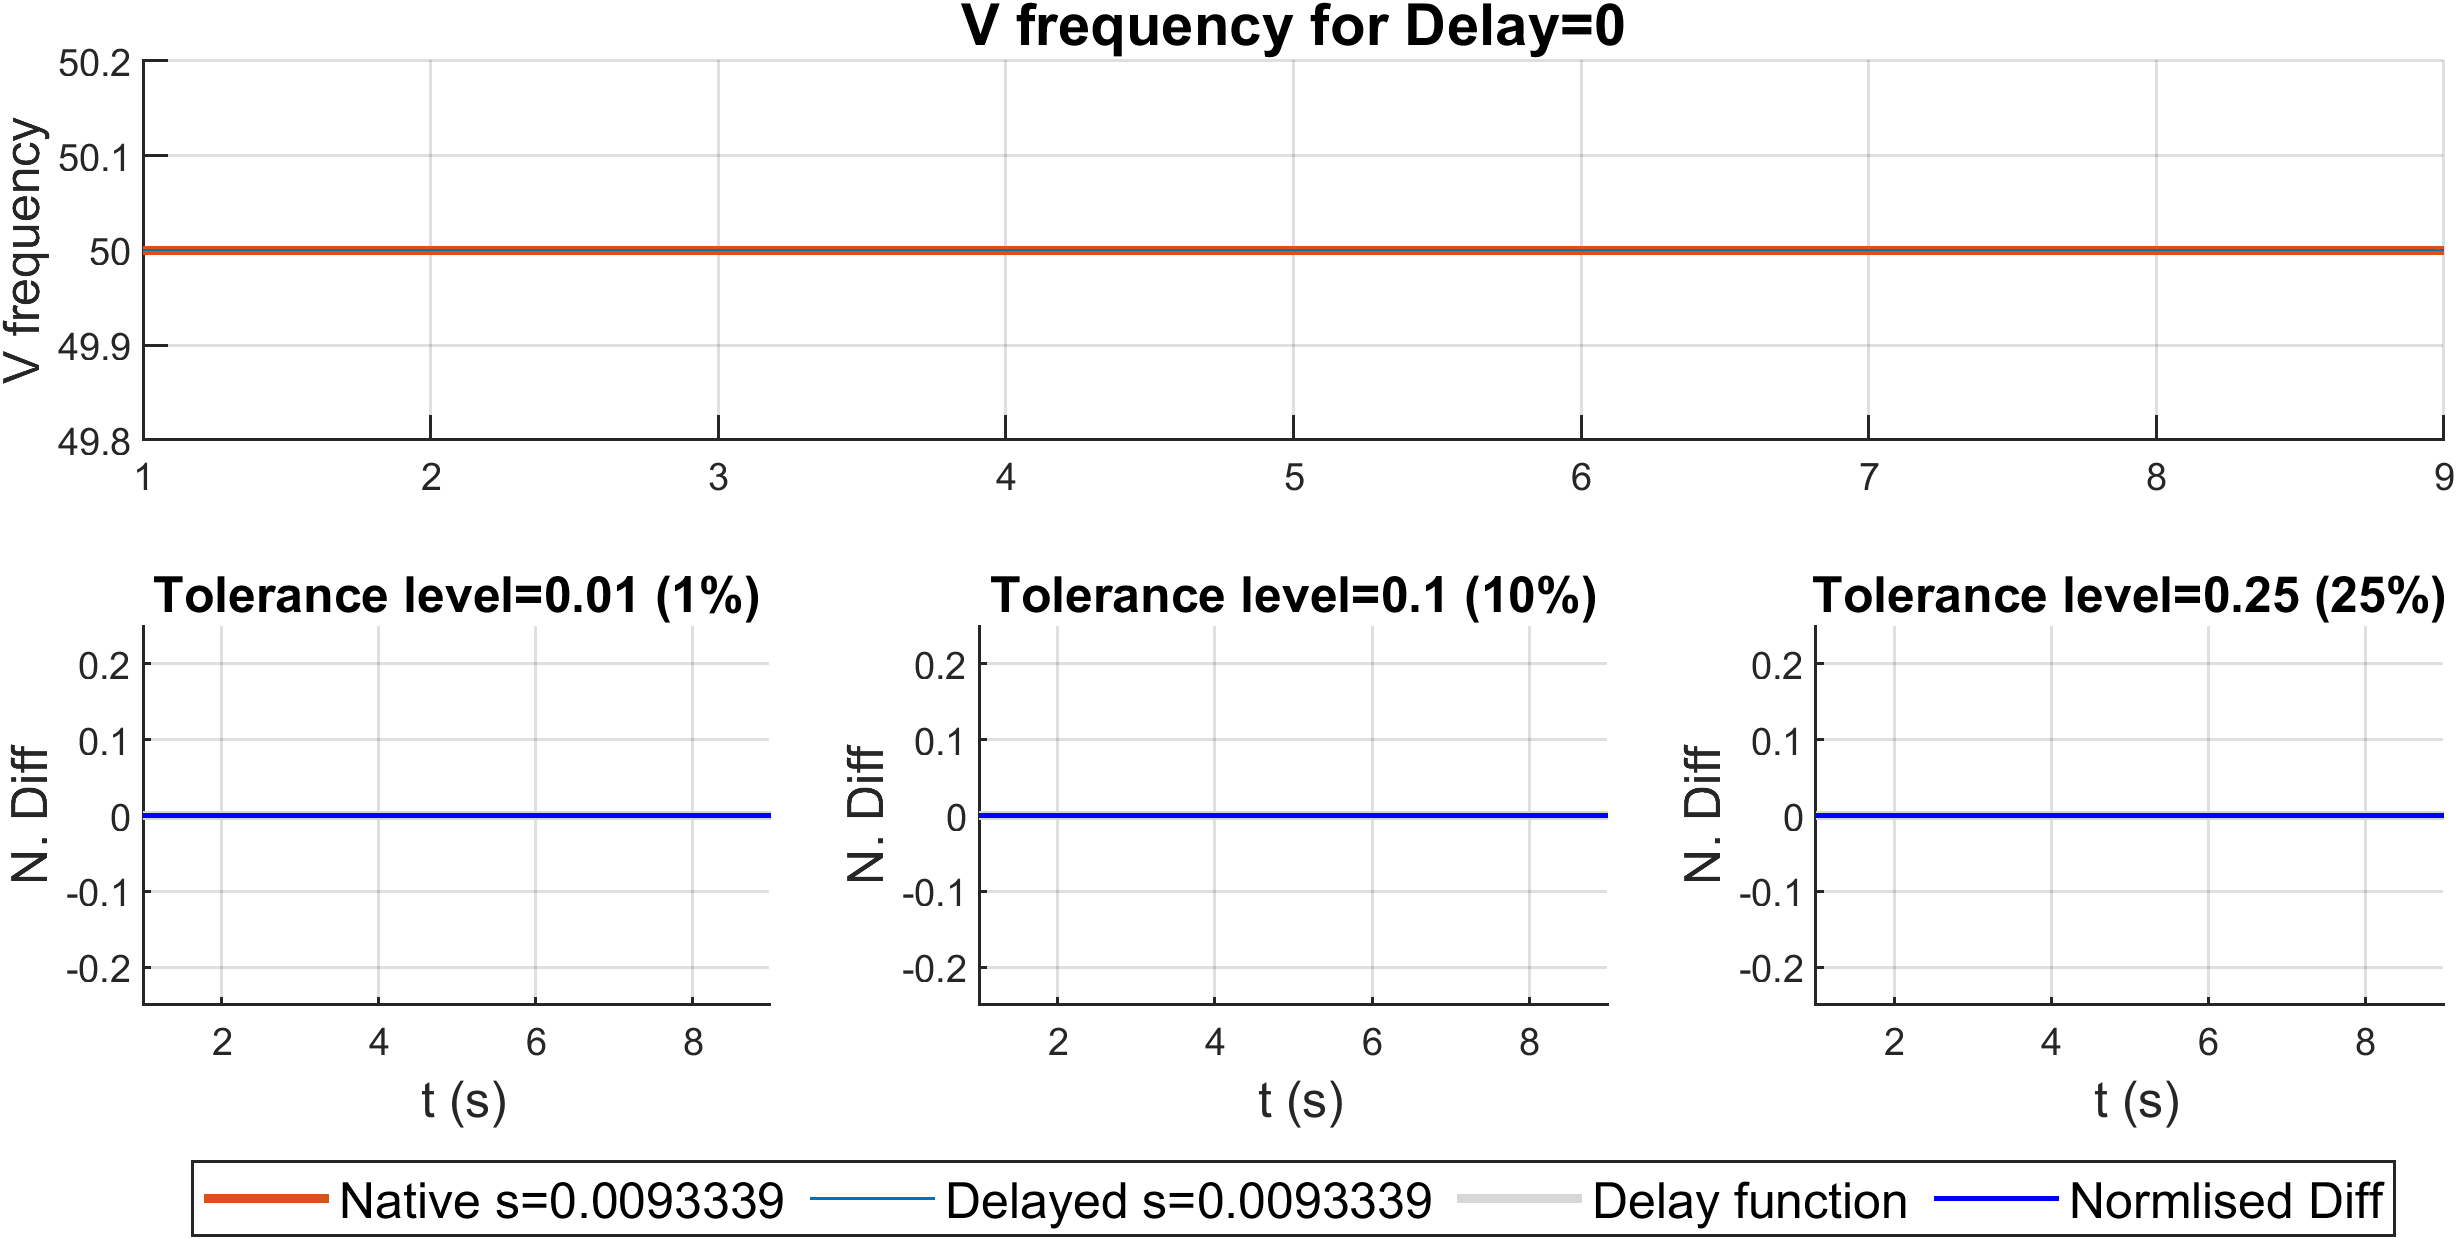
\includegraphics[width=0.95\textwidth]{\locateResults/DelayOf_0/Zero_vFrequency.png}    
    \caption{Ascending delay combined output}
    \label{fig:PMUsim_Zero_iFreq}
\end{figure}

\begin{figure}[hb]
    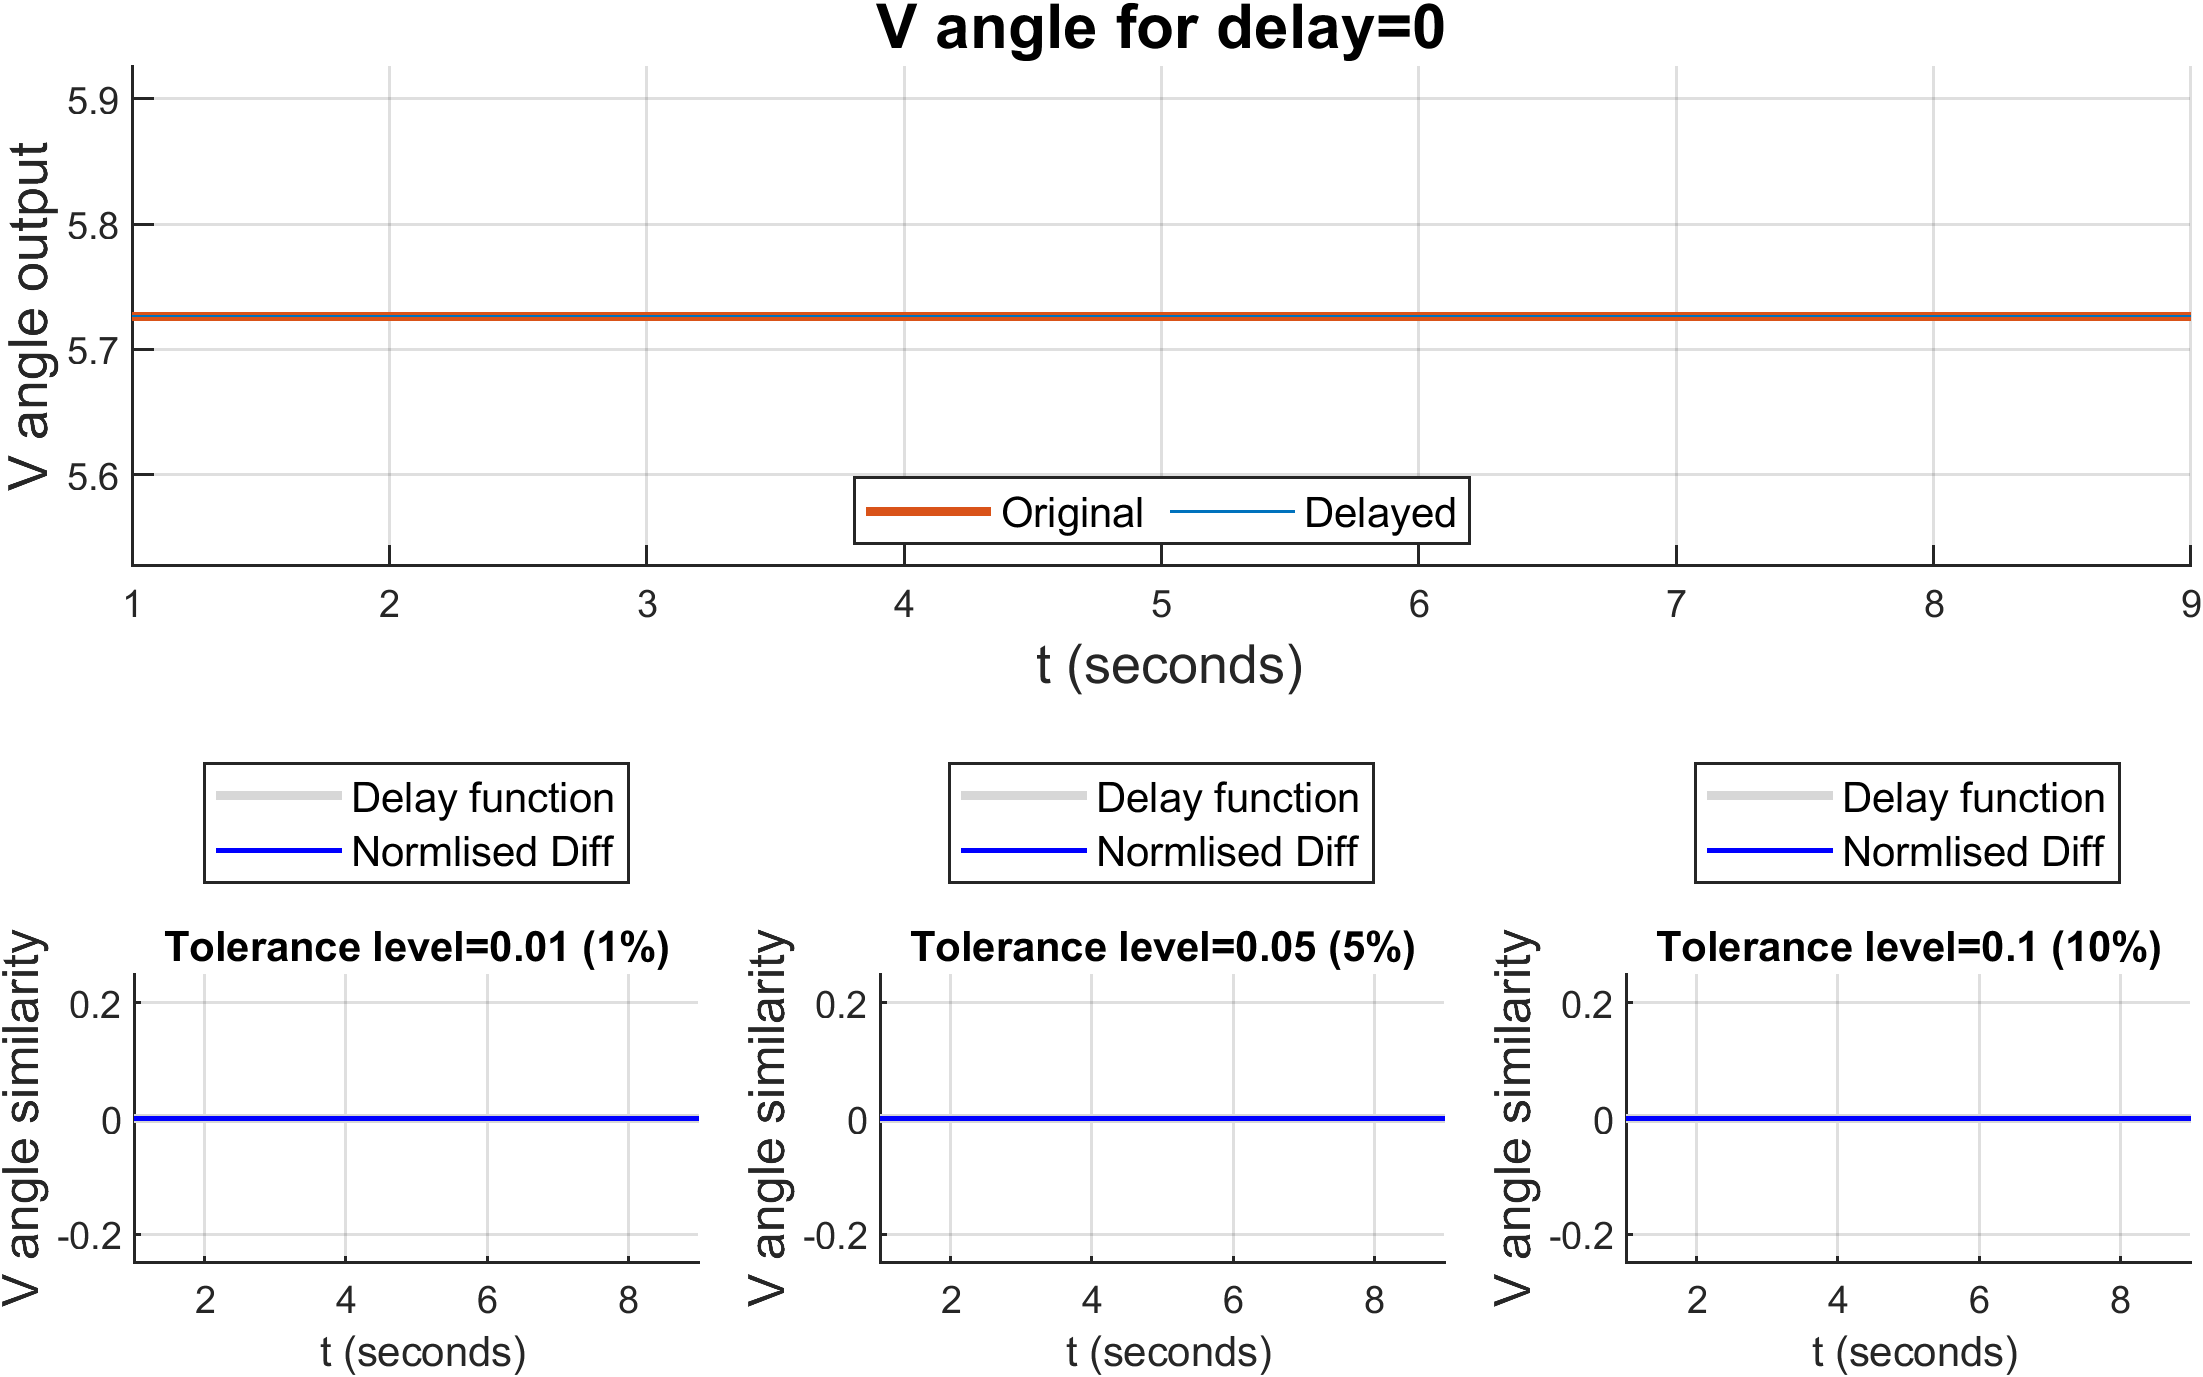
\includegraphics[width=0.95\textwidth]{\locateResults/DelayOf_0/Zero_vAngle.png}    
    \caption{Ascending delay combined output}
    \label{fig:PMUsim_Zero_iAngle}
\end{figure}
\subsection{Voltage}


\begin{figure}[hb]
    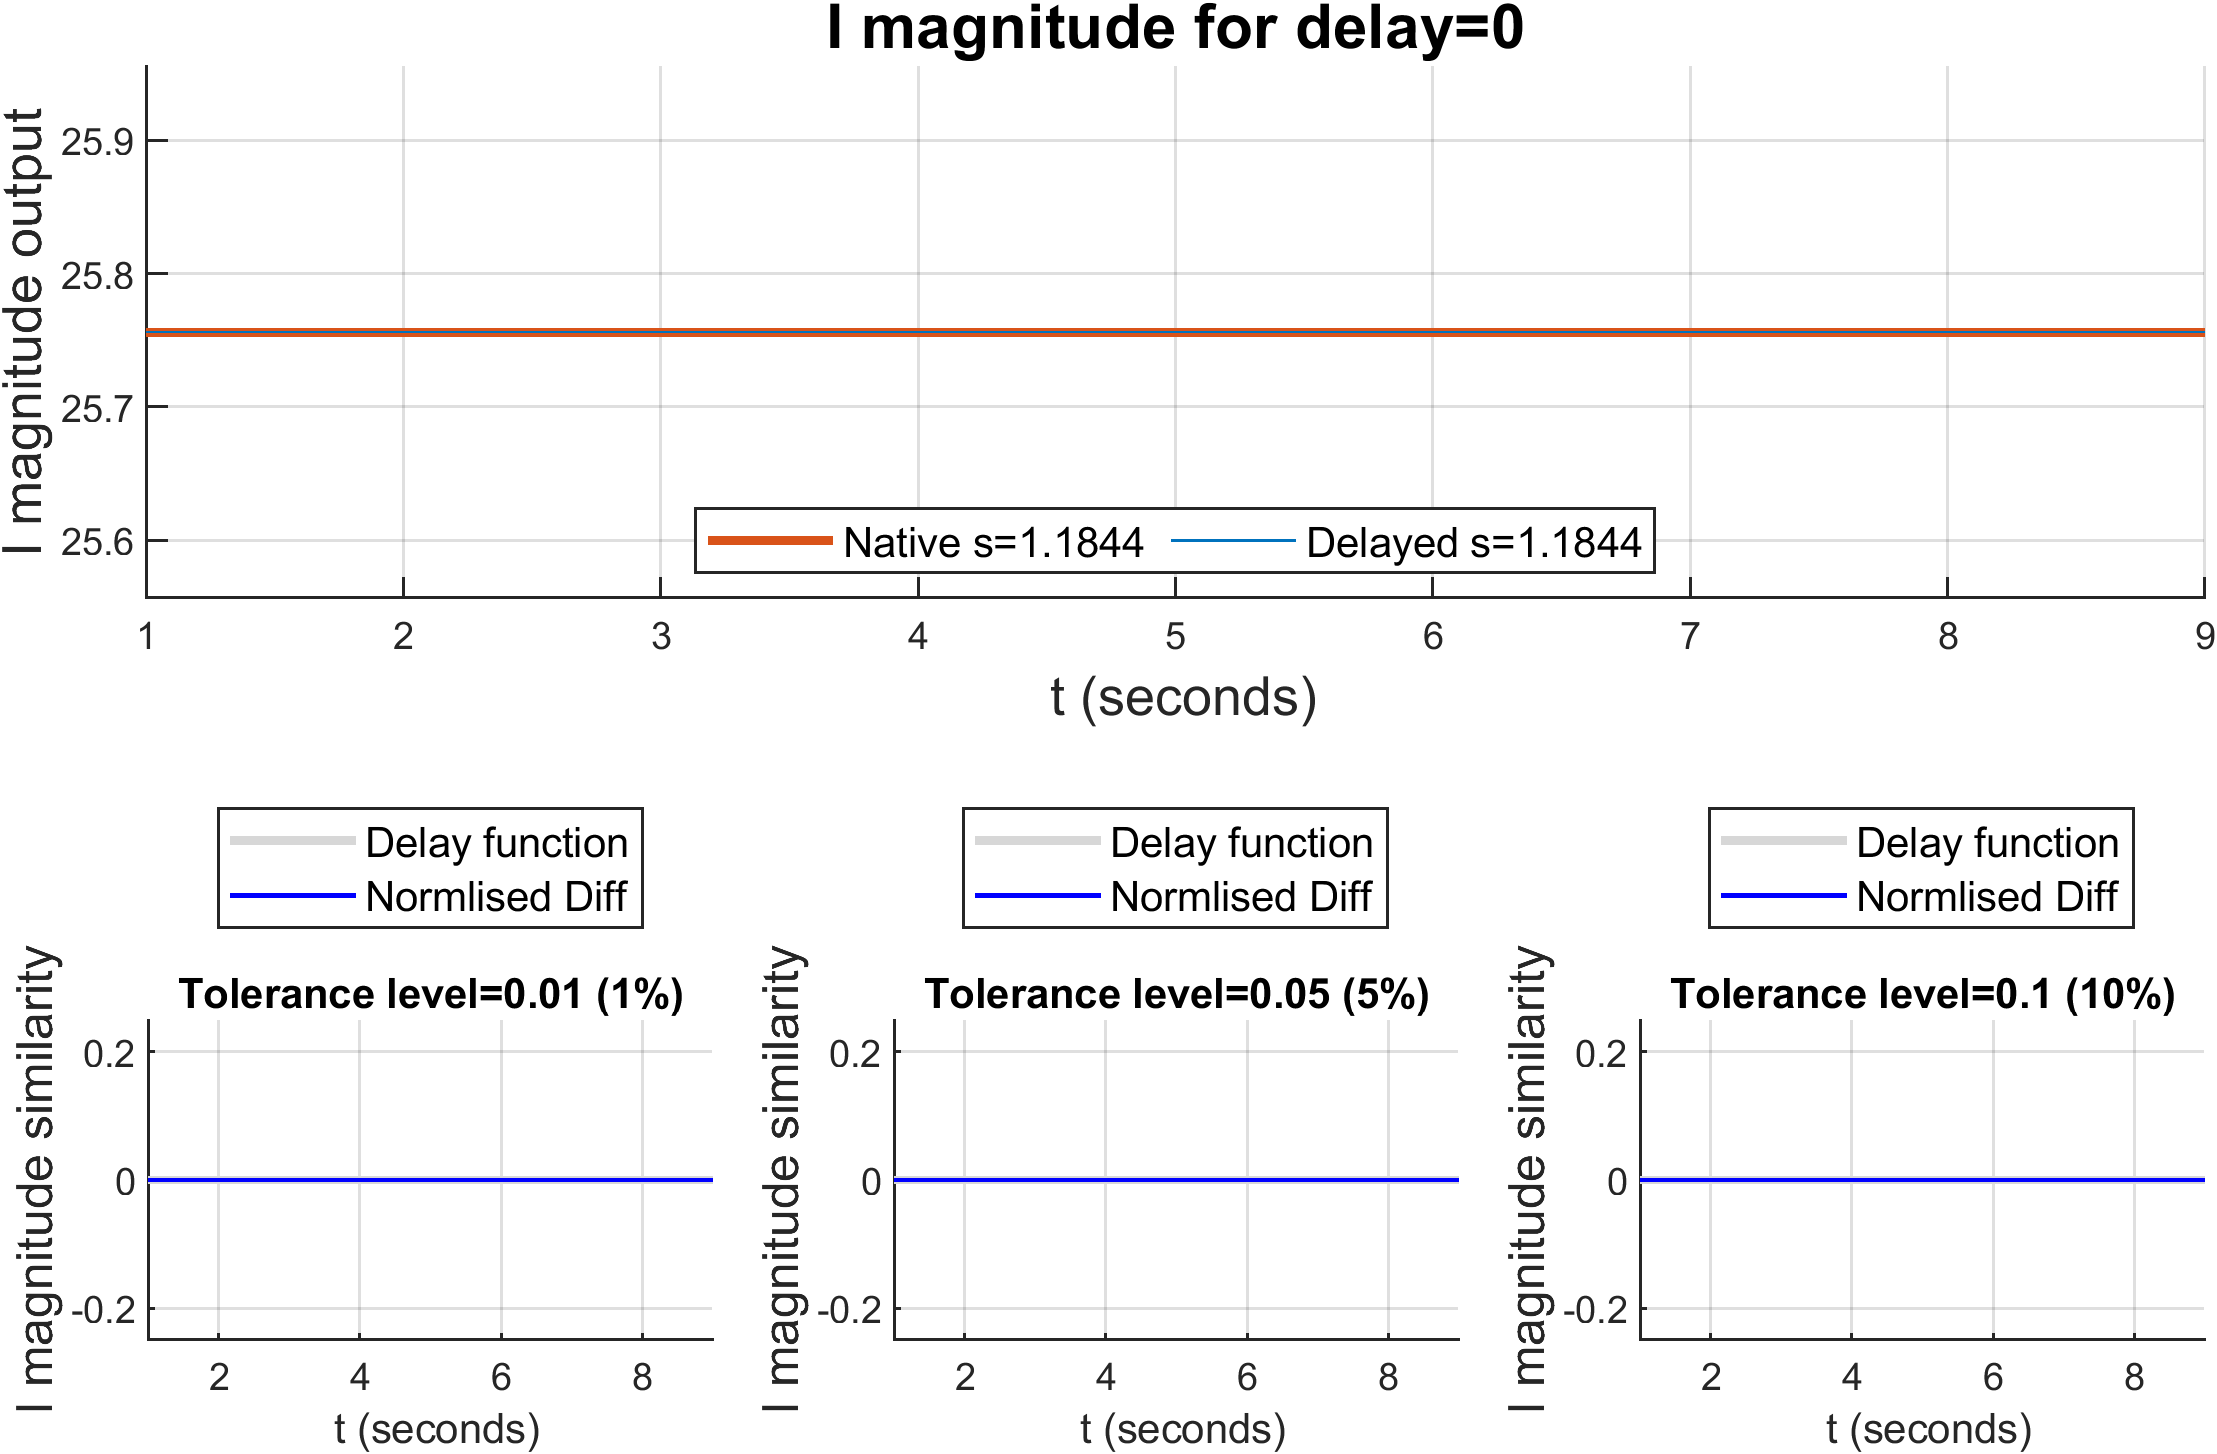
\includegraphics[width=0.95\textwidth]{\locateResults/DelayOf_0/Zero_iMagnitude.png}    
    \caption{Ascending delay combined output}
    \label{fig:PMUsim_Zero_iMagn}
\end{figure}

\begin{figure}[hb]
    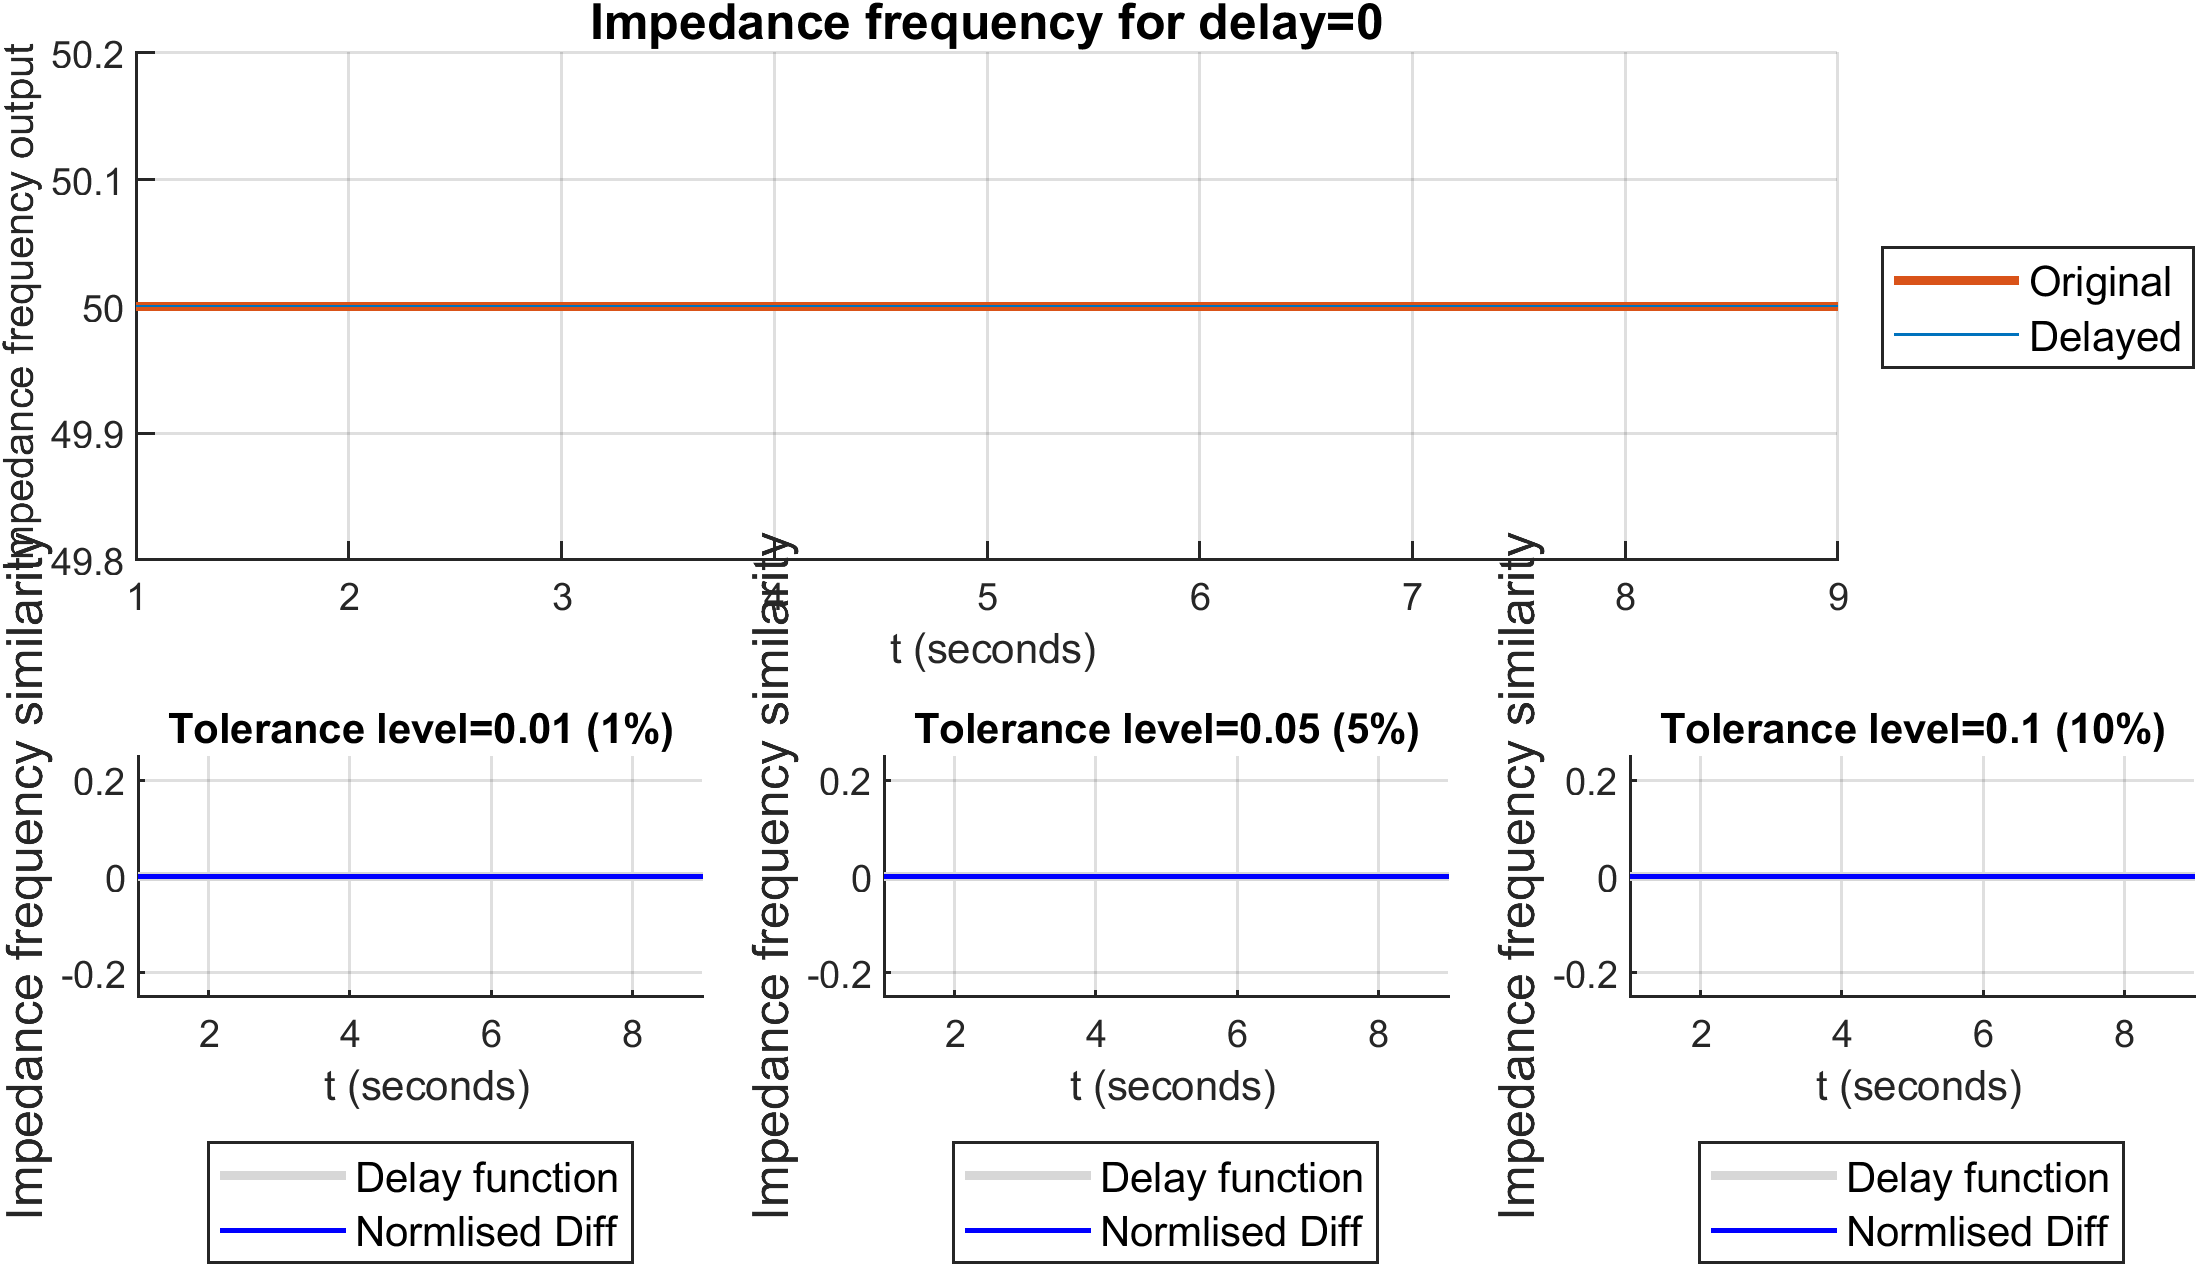
\includegraphics[width=0.95\textwidth]{\locateResults/DelayOf_0/Zero_iFrequency.png}    
    \caption{Ascending delay combined output}
    \label{fig:PMUsim_Zero_iFreq}
\end{figure}

\begin{figure}[hb]
    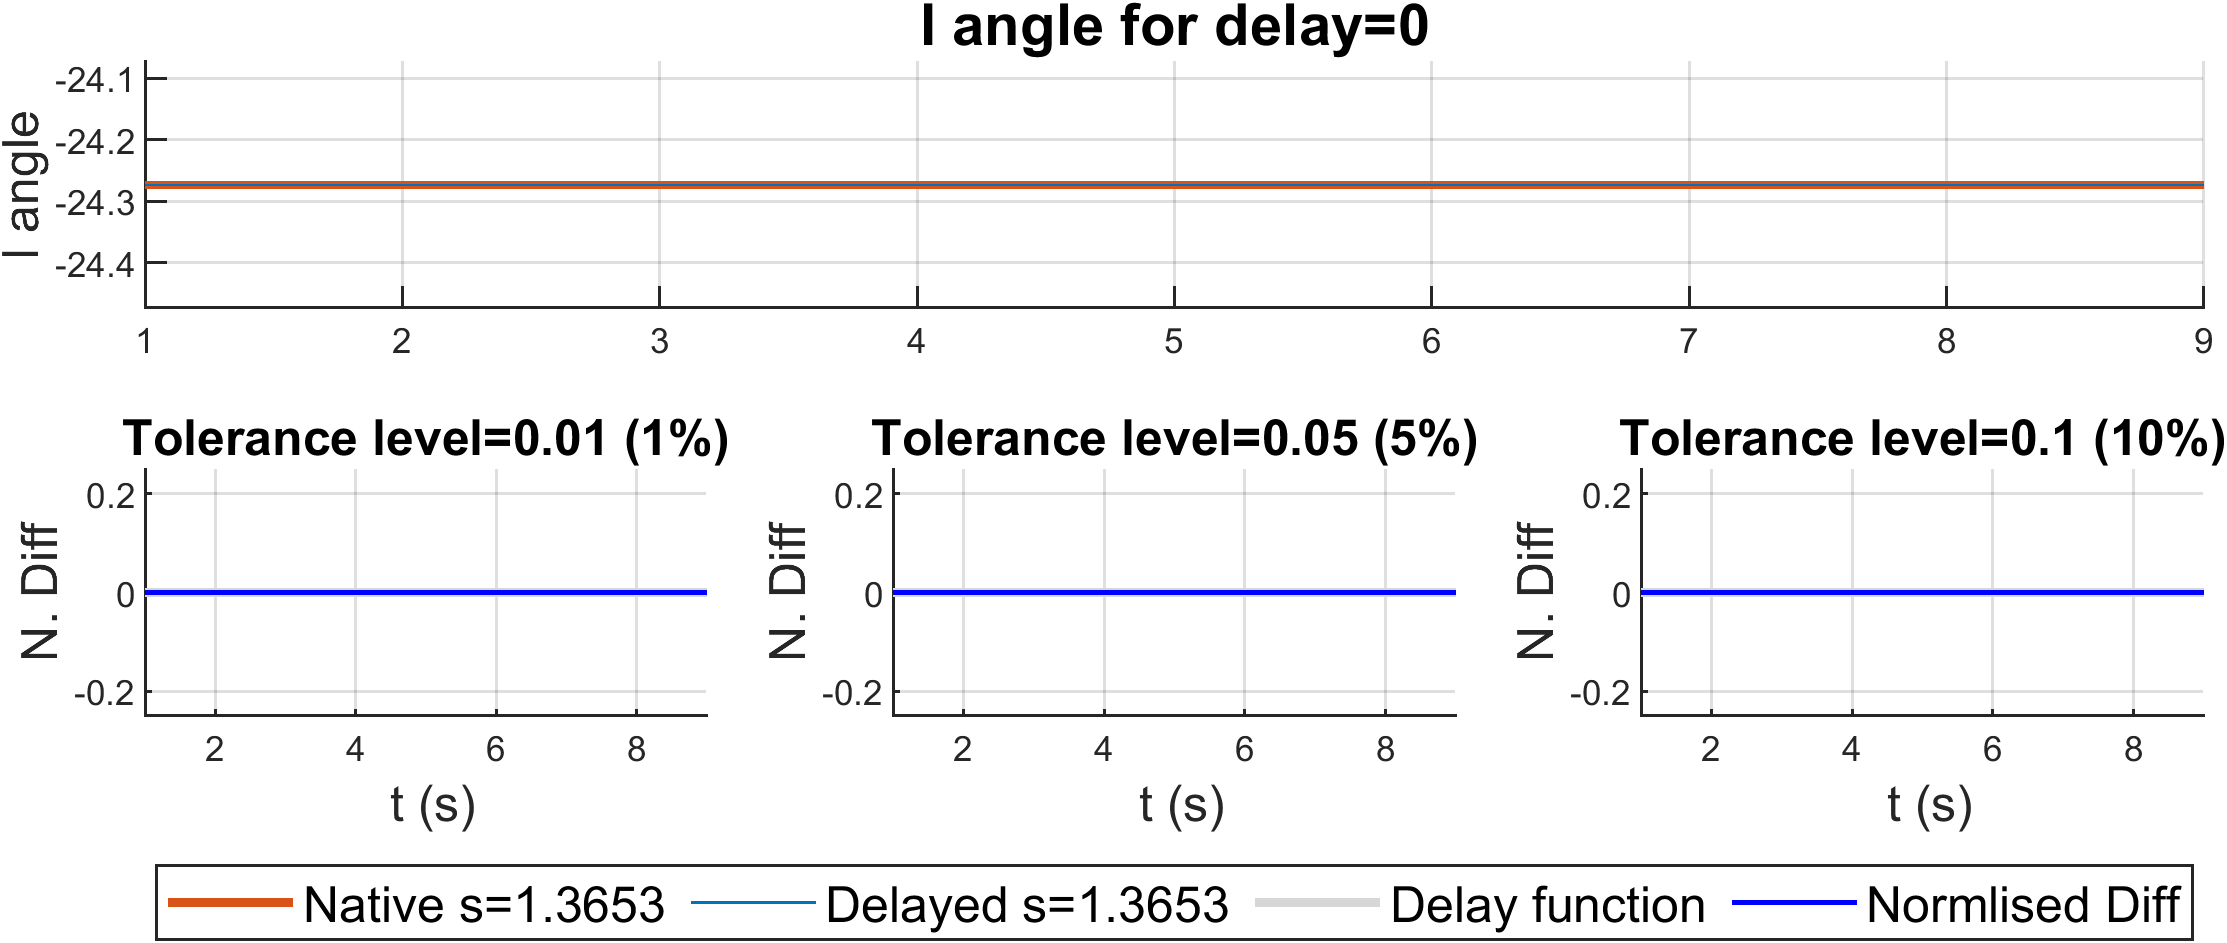
\includegraphics[width=0.95\textwidth]{\locateResults/DelayOf_0/Zero_iAngle.png}    
    \caption{Ascending delay combined output}
    \label{fig:PMUsim_Zero_iAngle}
\end{figure}

\subsection{Impedance}
